\chapter{Results and Discussion} \label{ch:results}

This chapter evaluates the model at three levels. First, the fixed biologically inspired pathways are tested without a trainable fusion readout. This establishes which localisation cues are already extracted by the hand-designed model, where calibration is required, and where the simplified pathways fail. Second, the direct and residual SNN fusion readouts are evaluated to determine whether trainable integration can correct predictable cross-cue errors. Third, these models are compared with input-only SNN baselines to test whether the biologically structured intermediate populations provide useful inductive bias.

The discussion is presented alongside the results. This is important because several effects are informative even when they reduce performance: the structure of a failure can show which cue has been lost, whether a later readout can recover it, and which simplifications should be revisited in future work.

\section{Evaluation Setup}

\subsection{Test Conditions}

The final experiments use the constrained operating region defined in Chapter~\ref{ch:modelling}: distance $r \in [0.25,5]$~m, azimuth $\theta \in [-45^\circ,45^\circ]$, and elevation $\psi \in [-45^\circ,45^\circ]$. Each trainable model uses 2000 training, 400 validation, and 400 held-out test samples.

Three acoustic conditions are compared:
\begin{enumerate}
    \item \textbf{Noise-free:} the received signal contains the dominant simulated target echo only.
    \item \textbf{Environmental noise:} additive white Gaussian noise is inserted before the binaural head-shadow and elevation-filtering stages, using the fixed 50~dB call-referenced noise floor described in Chapter~\ref{ch:modelling}.
    \item \textbf{Noise + delayed echoes:} the same environmental noise is combined with the controlled sequence of delayed copies described in Chapter~\ref{ch:modelling}.
\end{enumerate}

The third condition should not be interpreted as a realistic room-reverberation model. The delayed copies retain the same simulated target-dependent transformations and occur in the same order on every trial. This makes the condition useful as a controlled clutter stress test, but easier than a real scene in which reflections arrive from different surfaces, directions, and materials.

\subsection{Metrics}

Distance errors are reported in metres or centimetres and angular errors in degrees. Spherical predictions are also converted into Cartesian positions to compute Euclidean error,
\begin{equation}
    e_{\mathrm{3D},i}
    =
    \left\|
        \hat{\mathbf{p}}_i-\mathbf{p}_i
    \right\|_2 ,
\end{equation}
where $\mathbf{p}_i$ and $\hat{\mathbf{p}}_i$ are the true and predicted positions.

A dimensionless combined error is used to compare the three-coordinate readouts on one scale:
\begin{equation}
    e_{\mathrm{comb},i}
    =
    \frac{1}{3}
    \left(
        \frac{|\hat{r}_i-r_i|}{5~\mathrm{m}}
        +
        \frac{|\Delta\hat{\theta}_i|}{45^\circ}
        +
        \frac{|\Delta\hat{\psi}_i|}{45^\circ}
    \right),
\end{equation}
\begin{equation}
    E_{\mathrm{comb}}
    =
    \frac{1}{N}
    \sum_{i=1}^{N}
    e_{\mathrm{comb},i}.
\end{equation}
Angular differences are wrapped before their magnitudes are calculated. The combined error is not a physical accuracy measure; it is a balanced summary for comparisons within this constrained operating region.

Where confidence intervals are reported, they are bootstrap 95\% intervals over the held-out test set. Bootstrap intervals are used because the error distributions are not assumed to be Gaussian and can contain structured failure cases.

\section{Fixed Biologically Inspired Pathways}

\subsection{Calibration and Azimuth-Cue Selection}

The fixed pathways are first analysed without trainable fusion. This separates the contribution of the hand-designed auditory model from later corrections learned by the SNN.

Azimuth required an explicit choice between the ITD and ILD branches. In an isolated $\pm45^\circ$ test, the uncalibrated ILD readout gave $11.799^\circ$ MAE, while the ITD coincidence readout gave $1.891^\circ$ MAE. Applying an inverse-sigmoid calibration reduced the isolated ILD error to $0.982^\circ$. This strong isolated result is useful, but it does not transfer cleanly to the full three-dimensional problem: calibrated ILD increased to $6.175^\circ$ MAE in the clean constrained 3D test, whereas ITD gave $3.351^\circ$.

Figure~\ref{fig:calibration_context} explains the difference. The simulated head-shadow cue is nonlinear and its ILD mapping changes with distance. ILD is therefore not a pure azimuth coordinate once the full signal model is used. By contrast, elevation calibration transfers more closely from an isolated sweep to the clean 3D stress sweep. The fixed scalar azimuth estimate consequently uses ITD, but the trainable fusion readout receives both the ITD and ILD populations. This retains useful complementary level information without assuming that one distance-independent ILD warp is sufficient.

\begin{figure}[H]
    \centering
    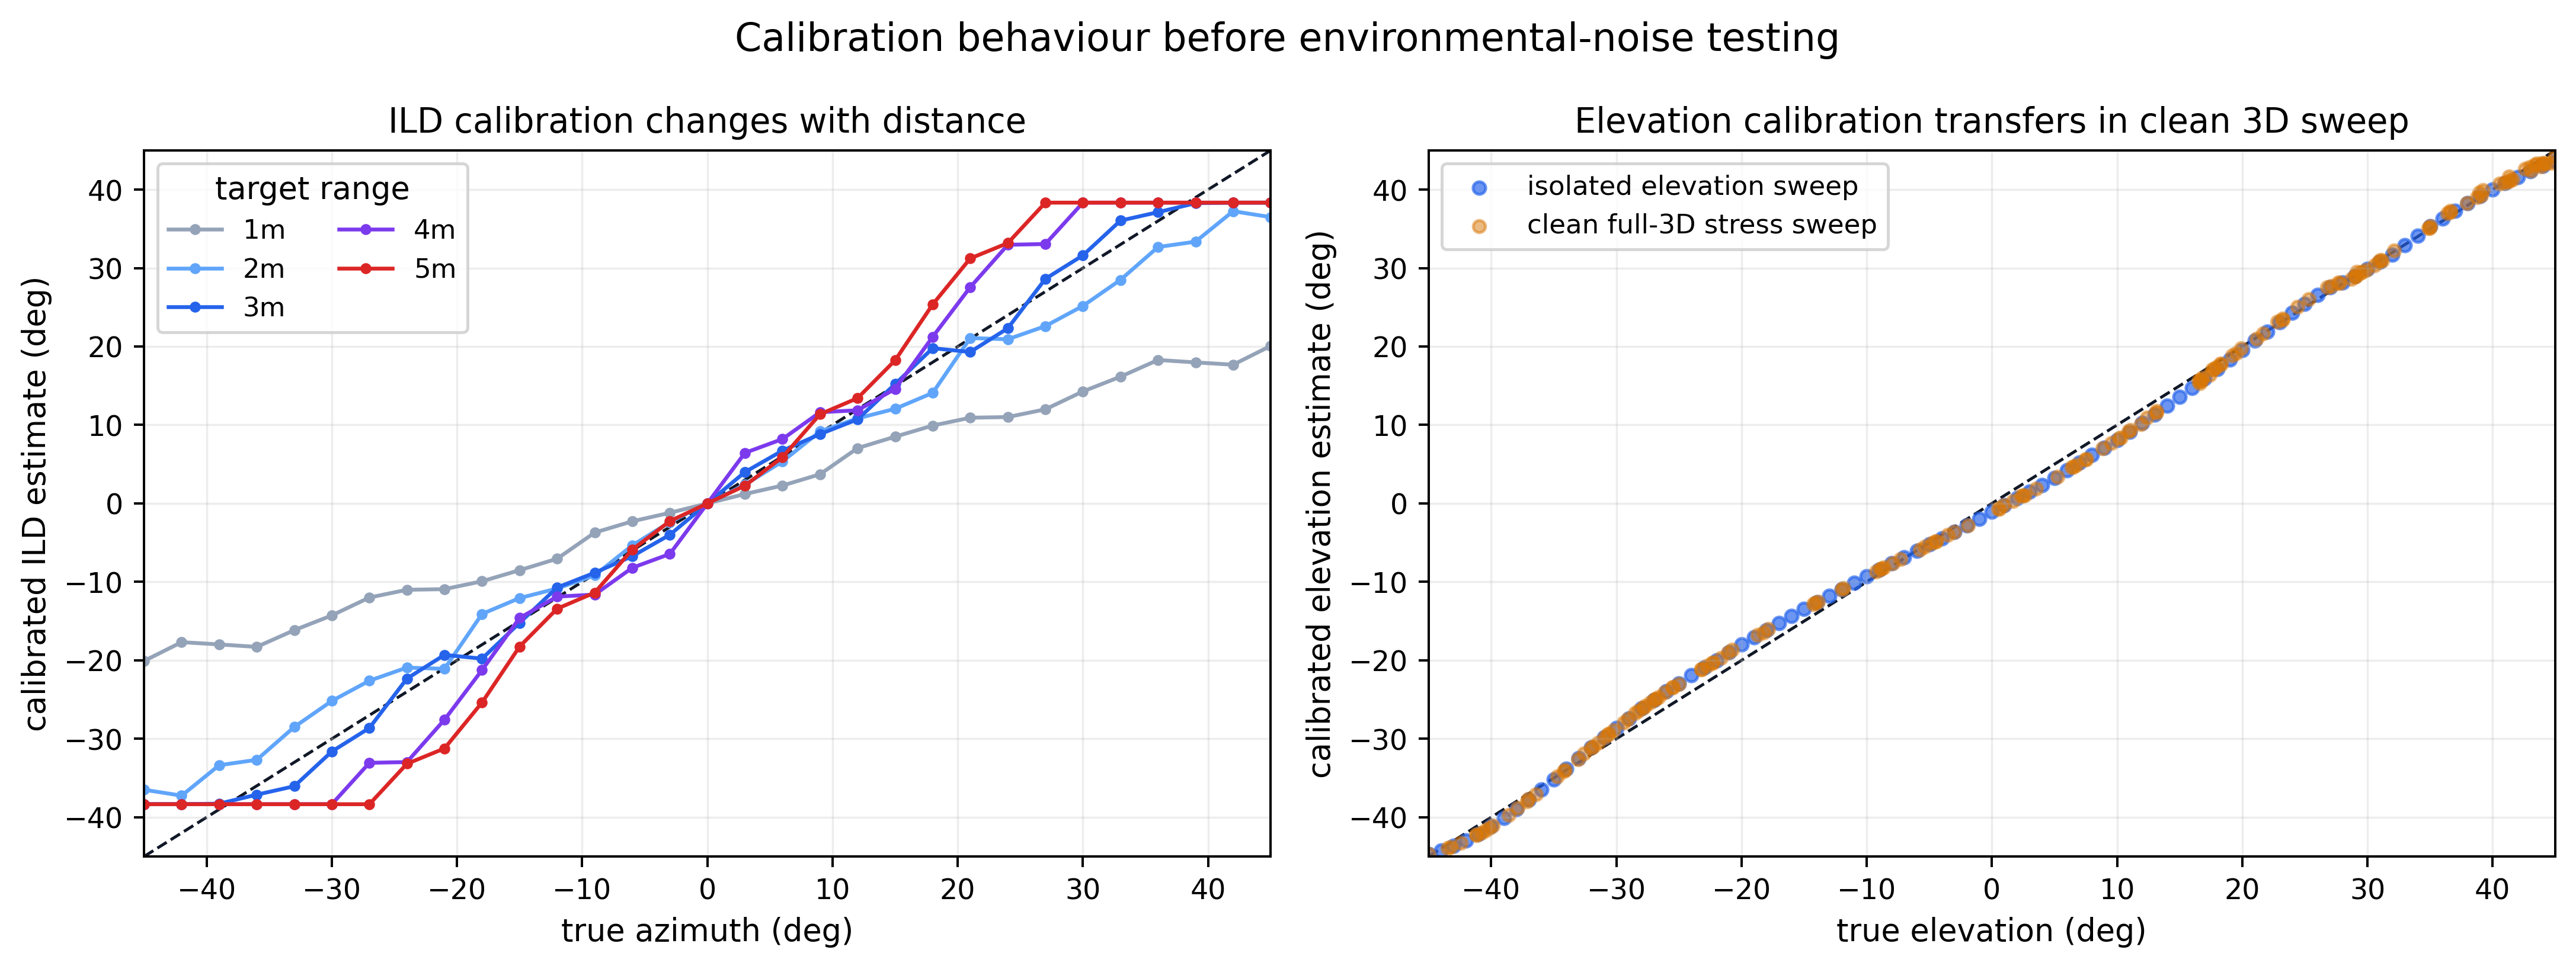
\includegraphics[width=0.95\textwidth]{4_Results/redraft_figures/02_calibration_context.png}
    \caption{Calibration context for the fixed pathways. Left: the simulated ILD mapping changes with distance, limiting a single azimuth calibration. Right: the inverse-sigmoid elevation calibration fitted on an isolated sweep transfers closely to the clean full-3D stress sweep. This clean transfer does not establish robustness to environmental noise.}
    \label{fig:calibration_context}
\end{figure}

\subsection{Fixed-Readout Results}

Table~\ref{tab:fixed_pathway_results} compares direct population decoding, calibrated direct decoding, and calibrated CANN decoding. Figure~\ref{fig:fixed_pathway_scatter} shows the corresponding scatter plots for the noise-free and full-noise conditions. The environmental-noise condition is omitted from the scatter figure to save space because its aggregate behaviour is very similar to the delayed-echo condition; it remains included in the numerical and binned-error comparisons.

\begin{table}[H]
    \centering
    \caption{Fixed-pathway results in the constrained three-dimensional test region. Values are coordinate MAEs. Calibration affects the elevation scalar readout; the fixed azimuth scalar is ITD-based.}
    \label{tab:fixed_pathway_results}
    \small
    \begin{tabular}{llrrrr}
        \toprule
        Condition & Readout & Distance & Azimuth & Elevation & Combined error \\
        \midrule
        Noise-free & Raw COM & 0.0365~m & 4.580$^\circ$ & 2.986$^\circ$ & 0.0585 \\
         & Calibrated COM & 0.0365~m & 4.580$^\circ$ & 1.336$^\circ$ & 0.0463 \\
         & Calibrated CANN & 0.0366~m & 4.925$^\circ$ & 0.910$^\circ$ & 0.0457 \\
        \midrule
        Environmental noise & Raw COM & 0.0786~m & 7.691$^\circ$ & 29.980$^\circ$ & 0.2843 \\
         & Calibrated COM & 0.0786~m & 7.691$^\circ$ & 27.961$^\circ$ & 0.2693 \\
         & Calibrated CANN & 0.0789~m & 8.094$^\circ$ & 26.642$^\circ$ & 0.2626 \\
        \midrule
        Noise + delayed echoes & Raw COM & 0.0796~m & 7.736$^\circ$ & 28.962$^\circ$ & 0.2771 \\
         & Calibrated COM & 0.0796~m & 7.736$^\circ$ & 27.203$^\circ$ & 0.2641 \\
         & Calibrated CANN & 0.0799~m & 8.147$^\circ$ & 25.975$^\circ$ & 0.2581 \\
        \bottomrule
    \end{tabular}
\end{table}

\begin{figure}[H]
    \centering
    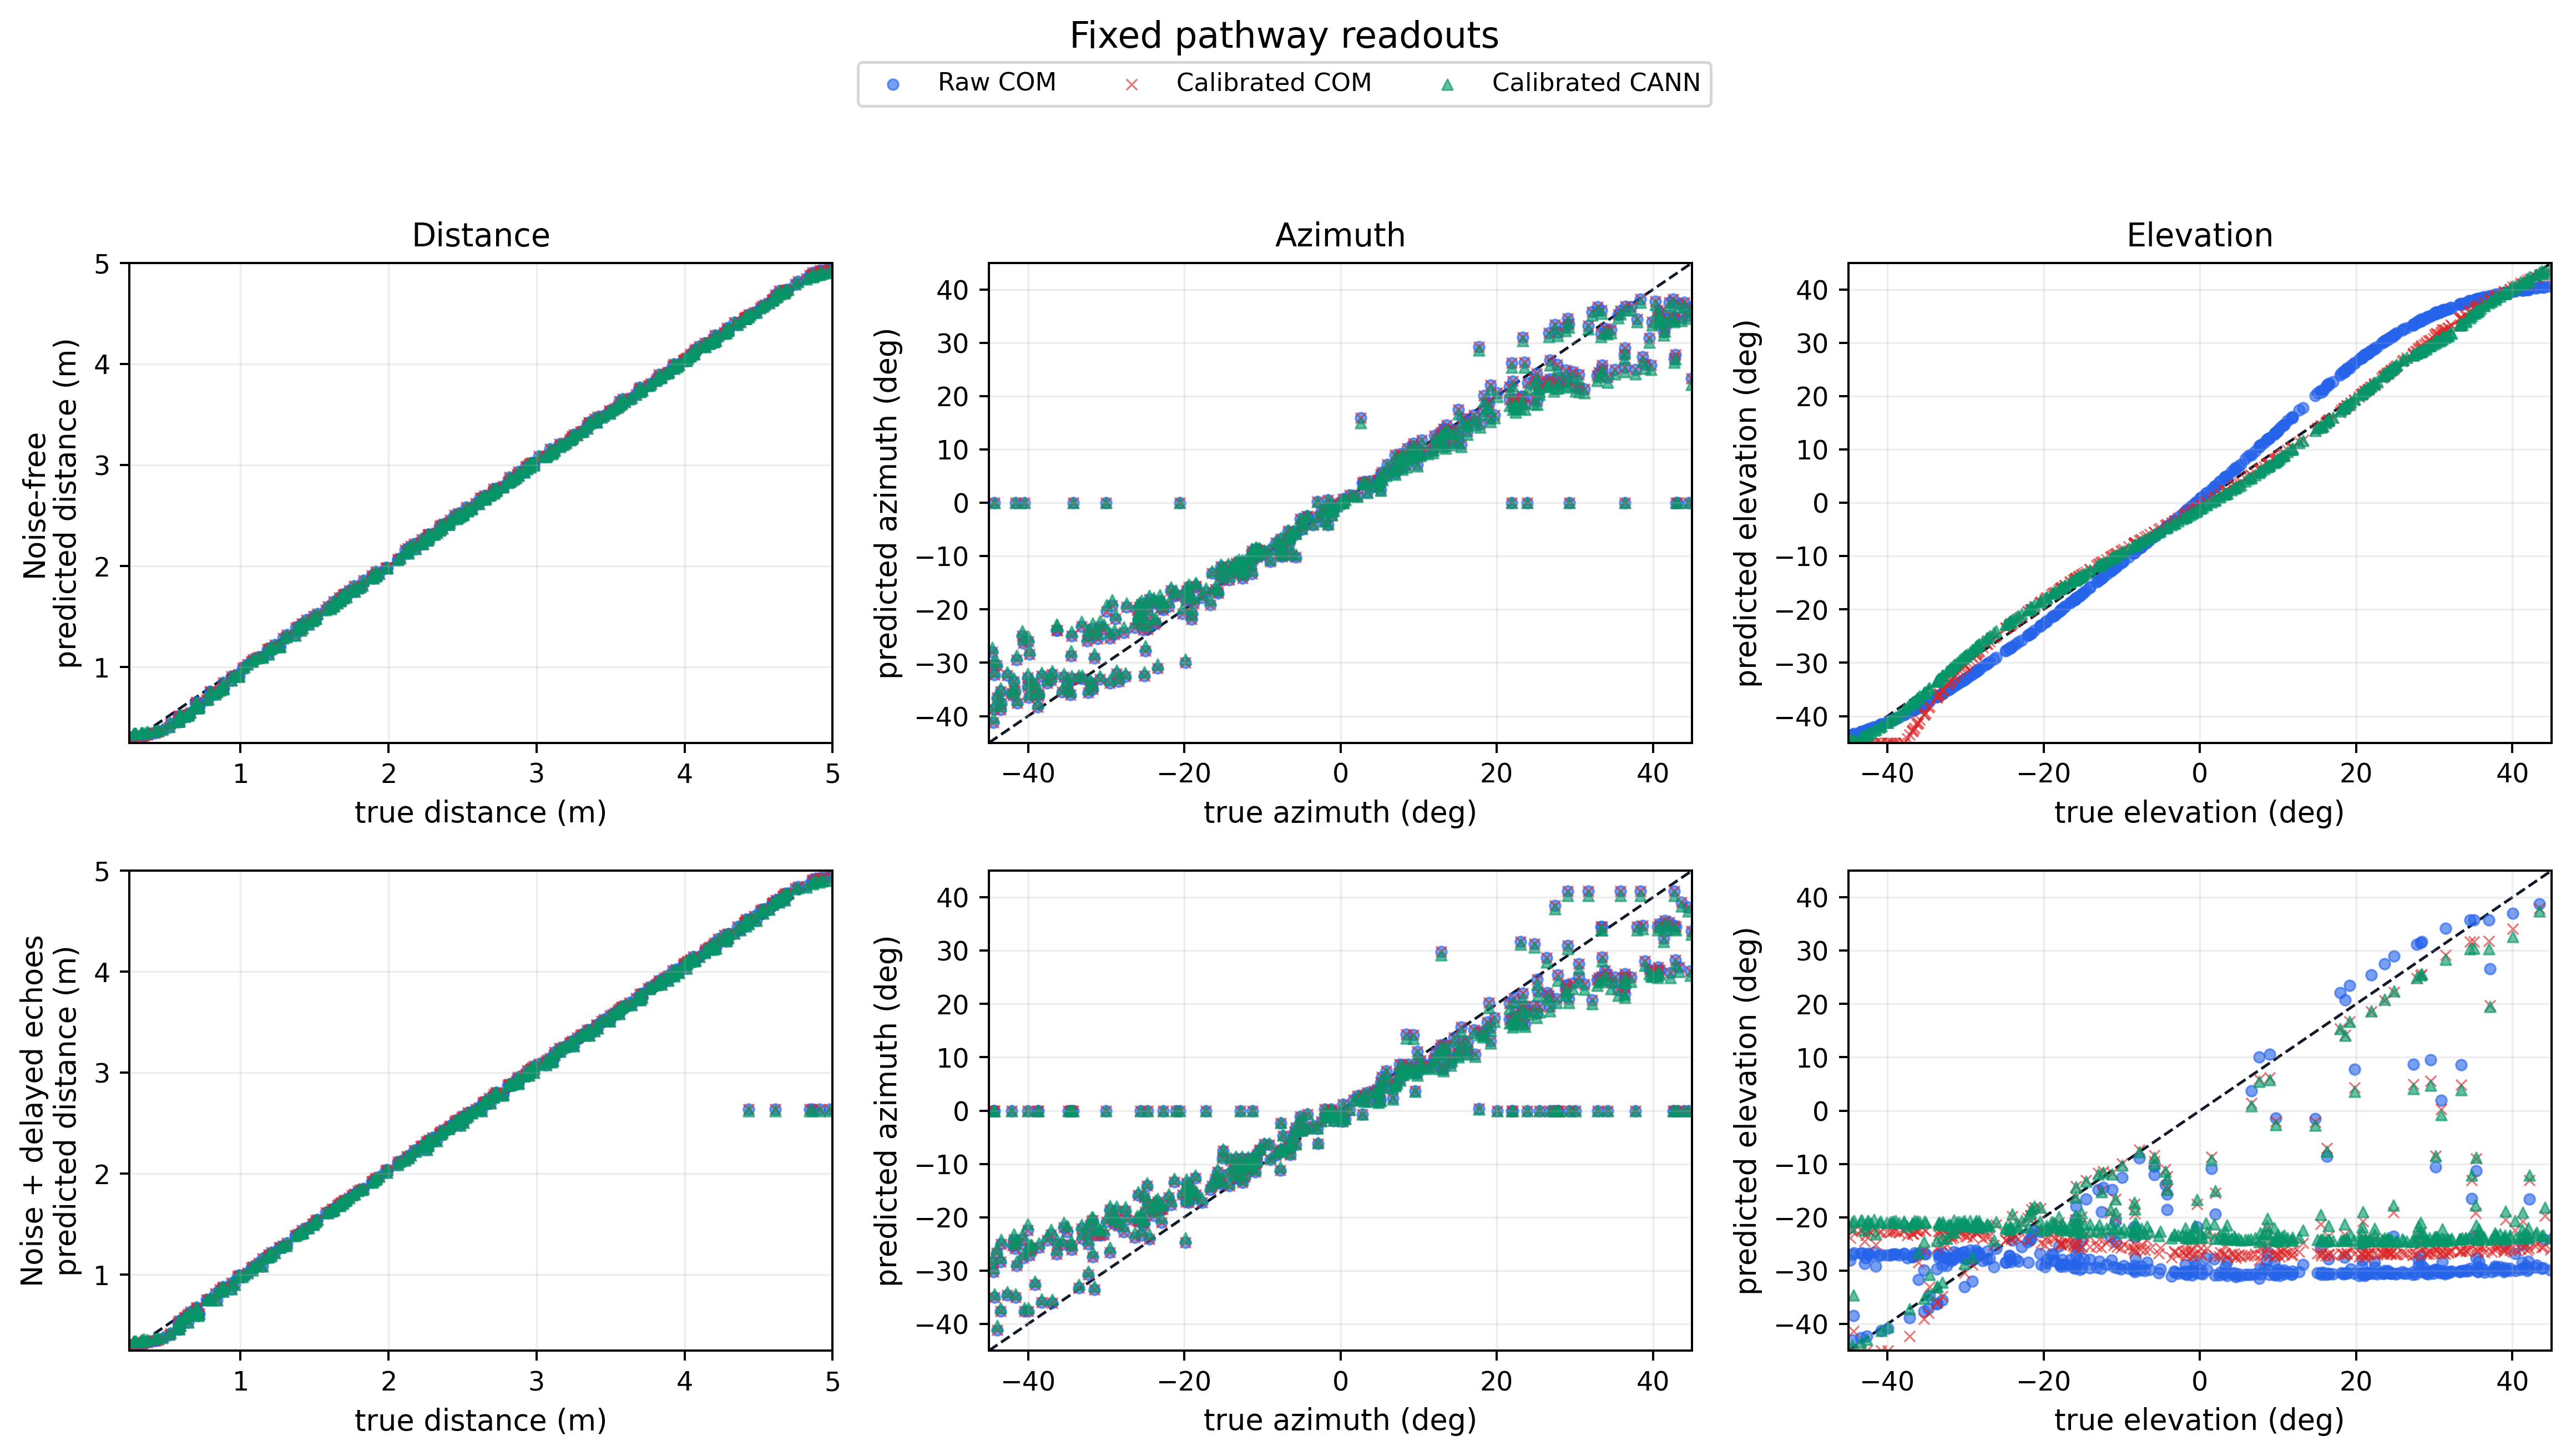
\includegraphics[width=\textwidth]{4_Results/redraft_figures/01_fixed_pathway_scatter.png}
    \caption{Fixed-pathway predictions before trainable fusion. Direct raw COM, calibrated COM, and calibrated CANN readouts are overlaid for each coordinate. The lower row uses environmental noise and delayed echoes.}
    \label{fig:fixed_pathway_scatter}
\end{figure}

The noise-free fixed model is already functional. Distance is the strongest raw pathway, with 3.65~cm MAE. Elevation calibration is also effective in the noise-free case, reducing elevation MAE from $2.986^\circ$ to $1.336^\circ$. Applying the CANN readout reduces it further to $0.910^\circ$. The improvement should be interpreted conservatively: calibration performs most of the correction, while the recurrent readout provides a smaller additional stabilisation.

The CANN is not a universal optimiser. Its clean azimuth MAE increases from $4.580^\circ$ to $4.925^\circ$, and distance is almost unchanged. This is consistent with the role proposed in Chapter~\ref{ch:modelling}: recurrence can stabilise an uncertain population and retain memory over time, but it cannot create information that is absent upstream. When a population is already sharp, smoothing can also introduce bias.

\subsection{Failure Structure}

Mean error alone hides where a pathway fails. Figure~\ref{fig:fixed_failure_curves} therefore bins raw fixed-pathway error by true coordinate. The three pathways exhibit distinct failure structures.

\begin{figure}[H]
    \centering
    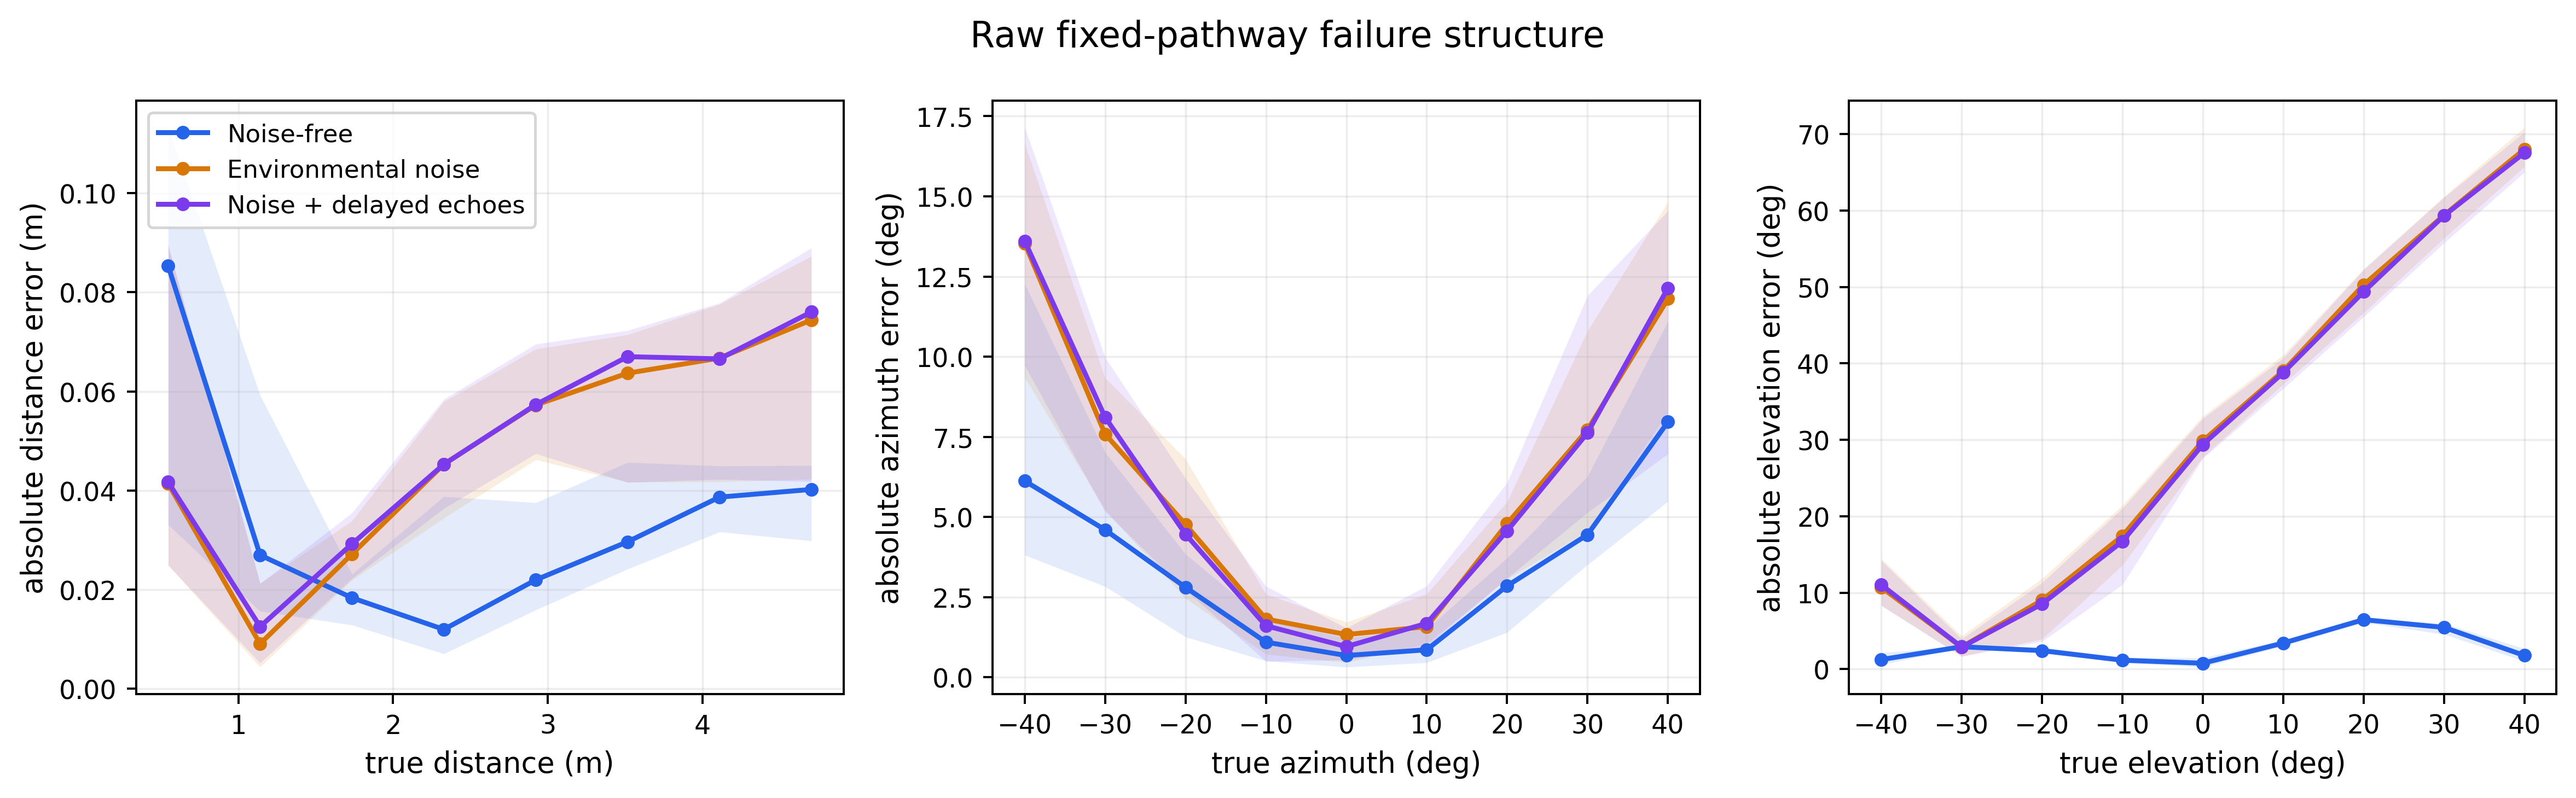
\includegraphics[width=\textwidth]{4_Results/redraft_figures/03_fixed_pathway_failure_curves.png}
    \caption{Coordinate-dependent absolute error of the raw fixed pathways. Lines show median error within coordinate bins and shaded regions show the interquartile range. All three acoustic conditions are included.}
    \label{fig:fixed_failure_curves}
\end{figure}

Distance remains comparatively stable, with failures concentrated at the far end of the range where attenuation makes the returned echo weakest. When the pathway fails, the estimate tends to fall back towards a short-range response. A plausible explanation is that the distance pathway benefits from the strongest explicit noise-control mechanisms in the model: VCN/VNLL onset consensus, DNLL-style suppression of late activity, and FM sweep facilitation in the IC. This remains a hypothesis rather than a causal conclusion. In the current implementation, the VCN stage already retains the first accepted event in each channel, so a clean DNLL ablation would require revising that upstream output before the independent contribution of suppression can be measured.

Azimuth degrades towards the centre of the field under noise. This is consistent with an ITD population losing reliable binaural onset differences: when evidence becomes weak or inconsistent across channels, the population becomes less directional and the COM estimate moves towards $0^\circ$. The delayed echoes slightly worsen the timing-based distance and azimuth pathways compared with environmental noise alone, although the difference is small.

Elevation fails differently. Under noise, predictions collapse towards a negative region rather than exactly to zero. A residual trend with true elevation is still visible within this collapse. This is important because it suggests that the cue has not disappeared completely: the DCN population retains some ordered information, but its clean calibration no longer matches the corrupted spectral profile. The high-elevation end is particularly difficult because the downward FM call contains less useful energy in the high-frequency region associated with those template notches. Signal weighting partly addresses this, but the remaining drop-off shows that the reliability correction is incomplete.

Adding delayed echoes slightly improves fixed elevation MAE, from $29.980^\circ$ to $28.962^\circ$ before calibration and from $26.642^\circ$ to $25.975^\circ$ after calibrated CANN decoding. This should not be interpreted as evidence that real reverberation helps elevation localisation. In this controlled simulator, the delayed copies retain target-consistent spectral shaping and can add repeated evidence. Real reflections would arrive with different directional filtering and would be less likely to reinforce the correct template.

\section{Trainable Fusion Readout}

The fixed-pathway failures motivate a trainable fusion stage. The direct SNN predicts coordinates from pathway features. The residual SNN starts from the fixed estimate and predicts a correction. Table~\ref{tab:trained_readout_results} gives the main results, with bootstrap intervals for the combined metric.

\begin{table}[H]
    \centering
    \caption{Fixed and trainable pathway-feature readouts. Brackets show bootstrap 95\% intervals for combined error over the 400-sample held-out test set.}
    \label{tab:trained_readout_results}
    \small
    \resizebox{\linewidth}{!}{%
    \begin{tabular}{llrrrrr}
        \toprule
        Condition & Readout & Distance MAE & Azimuth MAE & Elevation MAE & Euclidean MAE & Combined error \\
        \midrule
        Noise-free & Fixed calibrated CANN & 0.0366~m & 4.925$^\circ$ & 0.910$^\circ$ & 0.244~m & 0.0457 [0.041, 0.051] \\
         & Direct SNN & 0.0624~m & 2.449$^\circ$ & 1.133$^\circ$ & 0.161~m & 0.0307 [0.029, 0.033] \\
         & Residual SNN & 0.0139~m & 2.619$^\circ$ & 0.267$^\circ$ & 0.125~m & 0.0223 [0.020, 0.024] \\
        \midrule
        Environmental noise & Fixed calibrated CANN & 0.0789~m & 8.094$^\circ$ & 26.642$^\circ$ & 1.577~m & 0.2626 [0.246, 0.279] \\
         & Direct SNN & 0.0690~m & 3.831$^\circ$ & 4.018$^\circ$ & 0.321~m & 0.0627 [0.059, 0.067] \\
         & Residual SNN & 0.0213~m & 3.705$^\circ$ & 3.505$^\circ$ & 0.297~m & 0.0548 [0.051, 0.059] \\
        \midrule
        Noise + delayed echoes & Fixed calibrated CANN & 0.0799~m & 8.147$^\circ$ & 25.975$^\circ$ & 1.567~m & 0.2581 [0.242, 0.275] \\
         & Direct SNN & 0.0731~m & 3.883$^\circ$ & 4.028$^\circ$ & 0.343~m & 0.0635 [0.059, 0.068] \\
         & Residual SNN & 0.0202~m & 3.898$^\circ$ & 3.341$^\circ$ & 0.310~m & 0.0550 [0.050, 0.060] \\
        \bottomrule
    \end{tabular}%
    }
\end{table}

The residual SNN gives the lowest combined error in every condition. Its largest effect is on the fixed elevation breakdown: under environmental noise, elevation MAE falls from $26.642^\circ$ to $3.505^\circ$. Figure~\ref{fig:trained_scatter} shows that the trainable models correct most of the obvious collapse cases in the full-noise condition.

\begin{figure}[H]
    \centering
    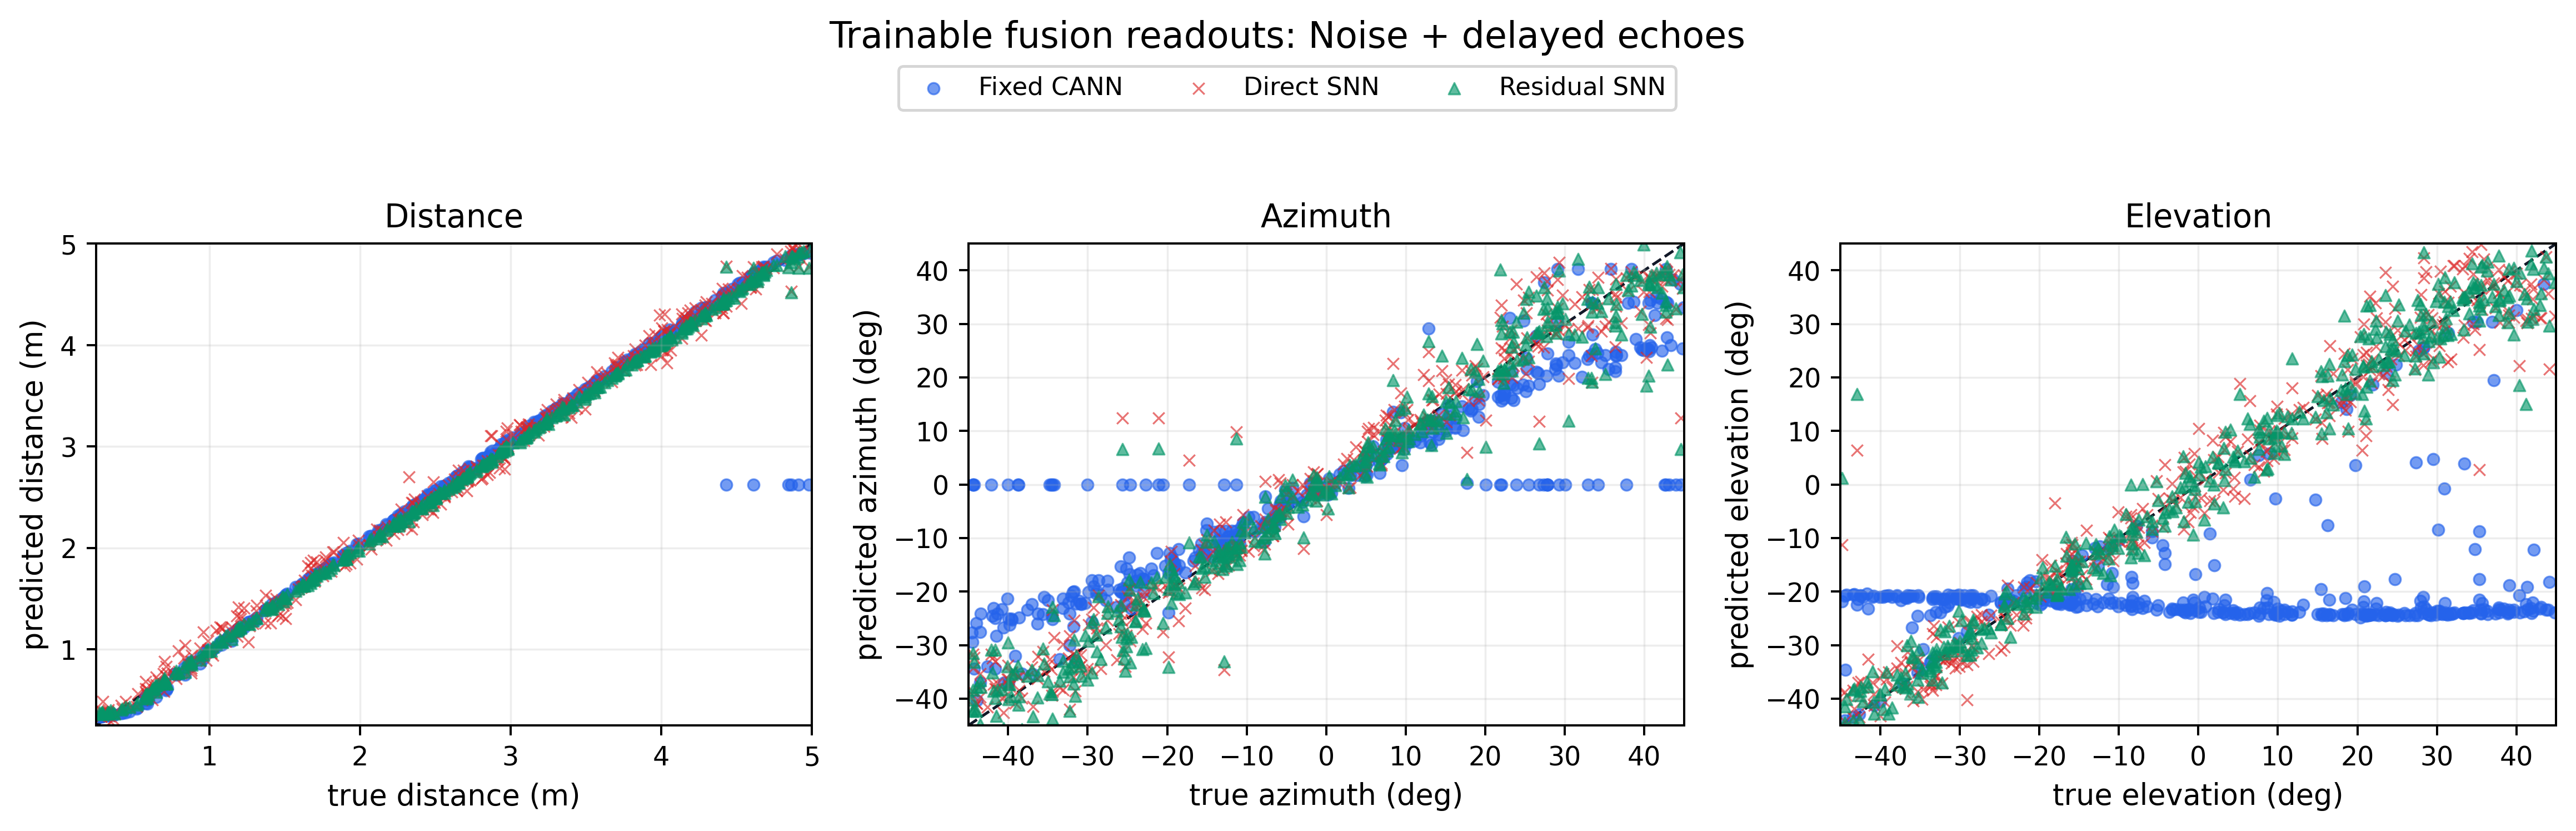
\includegraphics[width=\textwidth]{4_Results/redraft_figures/04_trained_fusion_delayed_echo_scatter.png}
    \caption{Fixed calibrated CANN, direct-SNN, and residual-SNN predictions with environmental noise and delayed echoes. The trainable readouts correct most of the fixed elevation collapse and substantially reduce the distance outliers.}
    \label{fig:trained_scatter}
\end{figure}

The correction is possible because failure does not imply complete information loss. Elevation predictions retain an ordered trend even during their noisy collapse, and the feature vector contains the full distance, ITD, ILD, and elevation populations rather than only three scalar estimates. The SNN can therefore learn systematic relationships between population shape, confidence, and coordinate error. Context from the stable distance population may be particularly valuable because attenuation and arrival-time reliability change with range.

This explanation has limits. The current fusion SNN receives a cached feature vector that is repeated across its simulation timesteps. It does not receive the original pathway spike trains as a temporally aligned stream. It therefore cannot literally learn to select an azimuth or elevation event because it arrived at the same time as the distance echo. Any benefit from echo timing is indirect: timing-derived structure has already been encoded into the cached pathway populations and confidence features. An explicitly temporal fusion architecture would be required to test the stronger time-alignment hypothesis.

Figure~\ref{fig:residual_failure_curves} shows the remaining residual-SNN error structure. The readout is much more stable than the fixed pathway, but its error is not uniform. Azimuth remains the least precisely resolved angular coordinate, and the Euclidean impact of angular error still increases with distance.

\begin{figure}[H]
    \centering
    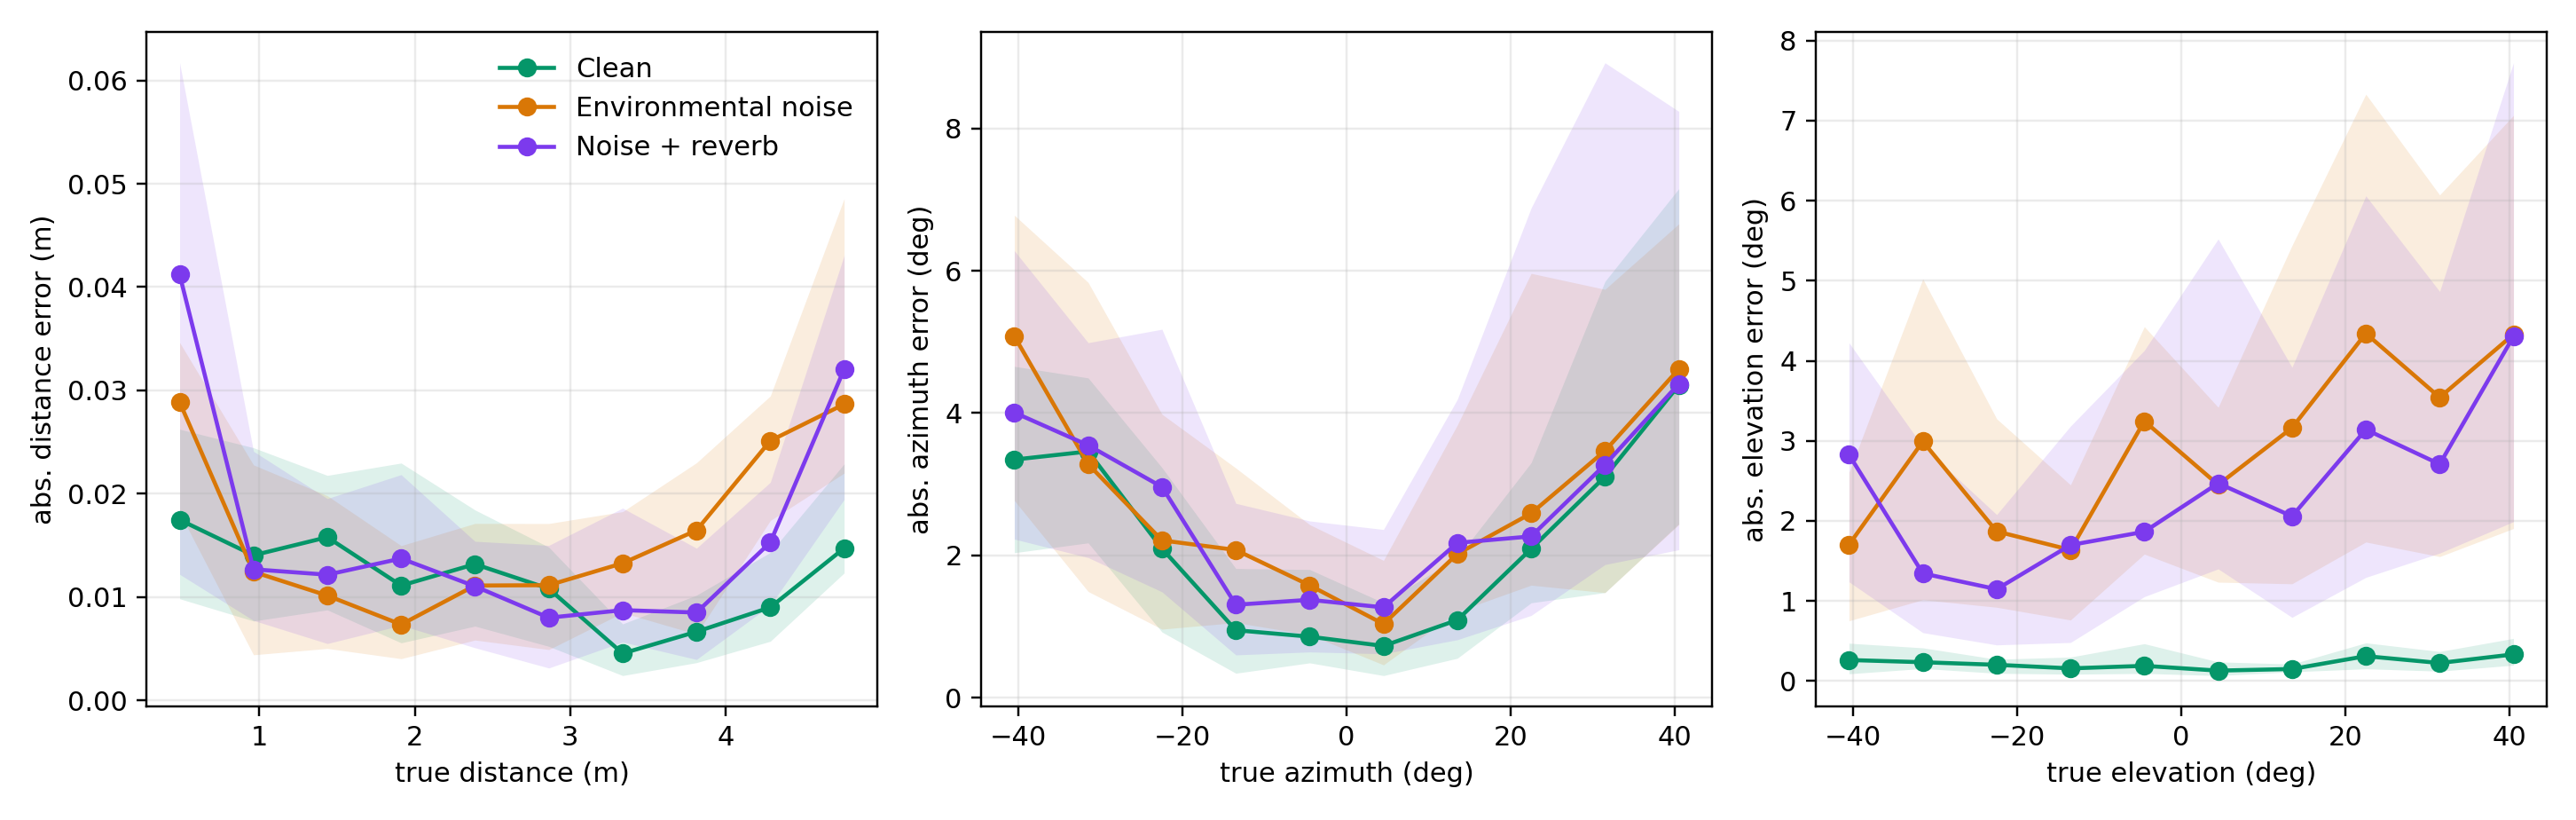
\includegraphics[width=\textwidth]{4_Results/trained/residual_binned_error_curves.png}
    \caption{Residual-SNN error structure across the coordinate range. Lines show median absolute error in coordinate bins and shaded regions show the interquartile range.}
    \label{fig:residual_failure_curves}
\end{figure}

\subsection{Feature Ablation}

Zero-ablation tests provide a more useful interpretation of the fusion model than first-layer weights alone. Figure~\ref{fig:feature_ablation} shows the change in combined error when each feature group is removed at test time.

\begin{figure}[H]
    \centering
    
\includegraphics[width=0.88\textwidth]{4_Results/redraft_figures/05_residual_feature_ablation.png}
    \caption{Residual-SNN feature-group ablation. Positive values indicate an increase in combined error when a feature group is zeroed at test time.}
    \label{fig:feature_ablation}
\end{figure}

The population features matter more than the three CANN scalar coordinates in isolation. This supports the use of population codes: a population retains peak width, ambiguity, margins, and off-centre activity that are lost when it is collapsed to one number. It also explains why the residual SNN can correct failures that the CANN scalar cannot. The readout has access to evidence about uncertainty, not merely a possibly biased estimate.

The ablation should still be interpreted carefully. Removing one feature group can move the input away from the distribution seen during training, and correlated groups can compensate for each other. The figure identifies useful dependencies, not a unique biological mechanism.

\section{Input-Only SNN Baselines}

The trainable readout must be compared with simpler trained models. Otherwise, improved performance could be attributed to adding any SNN rather than to the structured auditory pathways. Two input-only controls are therefore used. The waveform baseline receives flattened binaural waveform samples. The cochlear-raster baseline retains the cochlear front end but removes the cue-specific pathways. Table~\ref{tab:input_only_baselines} reports the direct variants; projected variants were also tested but are omitted here for space.

\begin{table}[H]
    \centering
    \caption{Direct input-only SNN baselines. These models use the same output target and loss structure as the fusion SNN but do not receive the hand-designed cue populations.}
    \label{tab:input_only_baselines}
    \small
    \begin{tabular}{llrrrr}
        \toprule
        Condition & Input & Distance MAE & Azimuth MAE & Elevation MAE & Combined error \\
        \midrule
        Noise-free & Raw waveform & 0.8053~m & 21.580$^\circ$ & 22.855$^\circ$ & 0.3828 \\
         & Cochlear raster & 0.0651~m & 6.033$^\circ$ & 7.178$^\circ$ & 0.1022 \\
        \midrule
        Environmental noise & Raw waveform & 0.9794~m & 23.847$^\circ$ & 23.836$^\circ$ & 0.4185 \\
         & Cochlear raster & 0.0699~m & 5.991$^\circ$ & 4.678$^\circ$ & 0.0837 \\
        \midrule
        Noise + delayed echoes & Raw waveform & 0.9414~m & 21.990$^\circ$ & 22.471$^\circ$ & 0.3921 \\
         & Cochlear raster & 0.0632~m & 5.900$^\circ$ & 4.704$^\circ$ & 0.0828 \\
        \bottomrule
    \end{tabular}
\end{table}

\begin{figure}[H]
    \centering
    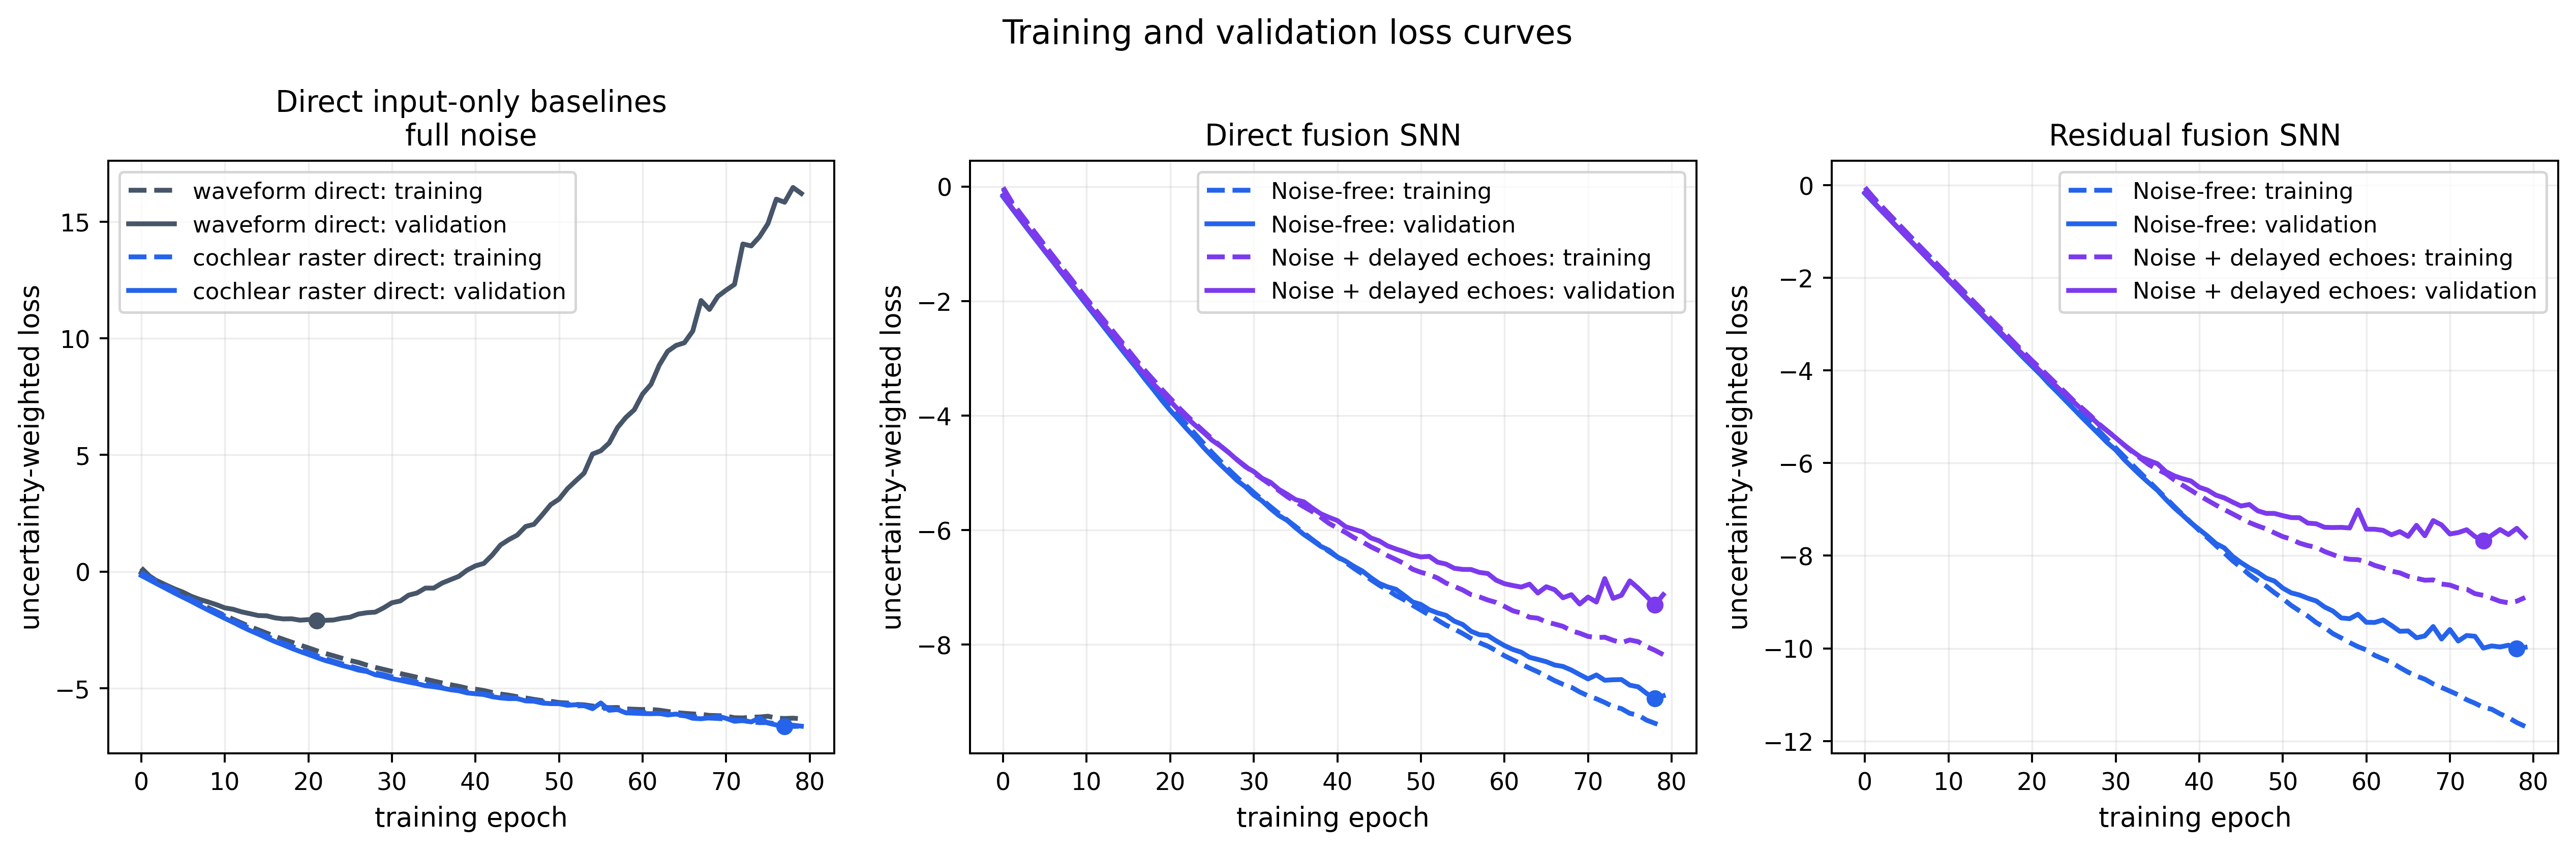
\includegraphics[width=\textwidth]{4_Results/redraft_figures/06_training_loss_curves.png}
    \caption{Training and validation losses. Left: direct input-only baselines. Centre: direct fusion SNN. Right: residual fusion SNN. Dashed lines show training loss, solid lines show validation loss, and markers indicate retained validation epochs.}
    \label{fig:training_losses}
\end{figure}

The direct raw-waveform baseline performs poorly despite receiving the least processed data. This is not evidence that continuous current injection into an LIF neuron is invalid: continuous input current is a standard modelling choice and is also used inside the cochlear encoder. The comparison instead shows that this small SNN and training set do not reliably discover the required filtering, timing comparison, and cue integration directly from flattened waveform features.

The cochlear-raster baseline is substantially stronger. This is an important result because it identifies frequency extraction and spike encoding as valuable preprocessing even before later biological abstractions are added. However, the interpretation should remain proportionate: a cochlear filterbank also performs a basic signal-processing operation that many engineered systems would include in another form.

The clean raw pathway COM also gives 0.0585 combined error, outperforming the strongest clean input-only variant tested, the projected cochlear-raster baseline at 0.0828. This matters because it shows that the hand-designed pathway itself is a useful foundation before trainable correction is added. Under noise, however, the fixed elevation pathway breaks down and the cochlear-raster baseline becomes stronger than the fixed pathway. The residual fusion stage is therefore needed to retain the benefits of explicit feature extraction while correcting its simplified failure modes.

The structured residual SNN gives lower combined error than the input-only controls. Under environmental noise, for example, the residual model gives 0.0548 combined error compared with 0.0837 for the direct cochlear-raster baseline. There is one useful nuance: under noisy conditions, the cochlear-raster baseline has slightly lower Euclidean MAE than the residual SNN even though its balanced combined error is worse. This occurs because Euclidean distance weights coordinate errors according to target geometry, while the combined metric deliberately weights the three coordinate tasks more evenly. The model ranking therefore depends on the deployment objective.

\section{Resolution and Biological Context}

The population spacing provides a useful reference for readout precision. Table~\ref{tab:population_resolution} compares bin spacing with clean-condition error. Values below the spacing are described as \emph{sub-bin precision}, not automatically as biological hyperacuity. COM decoding can interpolate across a distributed population even when no neuron is centred exactly on the decoded coordinate.

\begin{table}[H]
    \centering
    \caption{Population resolution and clean-condition readout error. Residual-SNN values are system-level results after fusion and should not be interpreted as the acuity of one pathway alone.}
    \label{tab:population_resolution}
    \small
    \begin{tabular}{llrrl}
        \toprule
        Coordinate & Population & Bin spacing & Clean fixed error & Clean residual error \\
        \midrule
        Distance & AC distance population & 2.65~cm & 3.66~cm & 1.39~cm \\
        Azimuth & MSO/ITD population & $1.00^\circ$ & $4.925^\circ$ & $2.619^\circ$ \\
        Elevation & DCN template population & $1.00^\circ$ & $0.910^\circ$ & $0.267^\circ$ \\
        \bottomrule
    \end{tabular}
\end{table}

The residual system achieves sub-bin precision for distance and elevation in the clean condition, while the fixed elevation readout is also slightly below its $1^\circ$ spacing. Azimuth does not achieve sub-bin error. These values show that population decoding preserves more information than a nearest-bin classifier, but they do not demonstrate that the model reproduces bat perception.

Biological measurements provide useful context rather than a directly matched benchmark. FM bats have been reported to discriminate echo-delay differences below 60~$\mu$s, corresponding to approximately 1~cm of range difference under a simple round-trip calculation \cite{Simmons1973TheBats}. Reviews of bat auditory behaviour discuss still finer, sub-millimetre ranging performance in specialised jitter experiments \cite{Ulanovsky2008WhatBrain}. Indicative angular scales are also only a few degrees: approximately $1$--$2^\circ$ for azimuth and approximately $3^\circ$ for elevation are useful order-of-magnitude comparators, with external-ear structure contributing to vertical localisation \cite{Ulanovsky2008WhatBrain,Lawrence1982EcholocationTargets}. The simulated model does not reproduce these behavioural protocols, and the reported system MAEs should not be presented as equivalent perceptual thresholds.

\section{Comparison with Related Systems}

Direct comparison with published systems is difficult because the tasks differ substantially. Many neuromorphic localisation papers estimate direction of arrival from passive sounds, use classifier accuracy rather than continuous coordinate MAE, or test a different acoustic geometry. Danneville et al.\ note that distance estimation is rarely studied in the neuromorphic localisation literature \cite{Danneville2024ASystems}. Table~\ref{tab:literature_context} therefore uses published figures as context rather than as a leaderboard.

\begin{table}[H]
    \centering
    \caption{Context from related localisation systems. Values for Dalmas et al.\ and Roozbehi et al.\ are reported by the review in \cite{Danneville2024ASystems}; their tasks are not directly matched to this project.}
    \label{tab:literature_context}
    \small
    \begin{tabular}{p{0.25\linewidth}p{0.25\linewidth}p{0.21\linewidth}p{0.23\linewidth}}
        \toprule
        Reference & Task and environment & Reported result & Relevance \\
        \midrule
        Dalmas et al., reported in \cite{Danneville2024ASystems} & Direction-of-arrival localisation using natural sounds in a quiet simulated setting & 71.3\% accuracy at $1^\circ$ resolution & Demonstrates fine angular bins, but uses classification accuracy rather than continuous 3D error. \\
        Roozbehi et al., reported in \cite{Danneville2024ASystems} & Simulated noisy localisation with a reservoir SNN & 69.8\% accuracy, $3.4^\circ$ MAE, and 0.38~m MAE & Provides a noisy trained-SNN comparator, but the array geometry and task differ. \\
        Matsuo et al.\ \cite{Matsuo2013EcholocationSound} & FM-echo localisation using model-based signal processing & Sub-millimetre ranging reported in a controlled simulation & Shows the precision available from idealised FM timing, while this project focuses on a spiking, modular pathway under noise. \\
        Moro et al.\ \cite{Moro2022NeuromorphicTransducers} & Physical ultrasonic localisation with resistive memories & Hardware demonstration of neuromorphic object localisation & Demonstrates physical feasibility, but is not a matched software-accuracy benchmark. \\
        This project & Simulated active 3D localisation with fixed pathways and residual SNN fusion & 1.39~cm, $2.619^\circ$, and $0.267^\circ$ clean MAEs; 0.0548 combined error with environmental noise & Tests whether explicit biological pathway structure is useful before trainable fusion. \\
        \bottomrule
    \end{tabular}
\end{table}

The comparison highlights the specific scope of this work. It is not intended to replace high-precision cross-correlation in a sterile ranging task, nor to claim the best result across incompatible localisation datasets. Its contribution is the integration of interpretable distance, azimuth, and elevation populations with a small trainable spiking readout.

\section{Overall Discussion and Limitations}

The results support a coarse-to-fine interpretation of the architecture. The fixed pathways perform most of the physically meaningful feature extraction: time-of-flight for distance, binaural timing and level comparisons for azimuth, and spectral-template comparison for elevation. The residual SNN then performs contextual correction where the simplified pathways interact. This division of labour is valuable because the trainable component is not asked to rediscover the entire signal-processing chain from raw samples.

Population codes are central to this result. A bat does not need to calculate an explicit COM value, and the COM equations in this report should be understood as engineering readouts rather than literal perceptual models. The useful biological idea is that a distributed population retains graded and ambiguous evidence. Passing those populations into the fusion network preserves information that would be discarded by three scalar coordinates.

Preliminary mini-model experiments also provide limited support for explicitly encoding known structure. When delay-bank values were made trainable, they organised into a tonotopic delay map close to the fixed hand-designed values. This observation is not treated as a final benchmark because it was not rerun under the final evaluation protocol. It nevertheless motivates a controlled future comparison between fixed, learned, and biologically initialised delay maps.

The model also has clear limitations. The acoustics are synthetic; the delayed echoes are controlled copies rather than geometry-dependent reflections; the test region is constrained; the target is singular; and no measured HRTFs, surface materials, diffuse reverberation, or moving scenes are included. The fixed elevation pathway remains vulnerable when noise corrupts its spectral cue. The residual SNN corrects much of this vulnerability, but its internal strategy is not directly interpretable. The proposed explanations are hypotheses supported by error structure and ablation results, not proven neural mechanisms.

A useful next experiment is a causal pathway-ablation study. DNLL suppression and FM sweep facilitation should be removed independently and together using shared test signals, after revising the upstream first-onset representation so that late activity remains available for suppression. A second priority is an explicitly temporal fusion model that receives aligned pathway spike trains. This would test whether timing coincidences across pathways provide additional robustness beyond the cached population features used here.

The broader design argument is analogous to the motivation for physics-informed neural networks: a known structure can be built into a learned model rather than left to be rediscovered from data. The term biologically informed SNN (BI-SNN) is used here as a project-level description, not as an established model class. Within this simulated study, the approach occupies a useful middle ground between detailed biological modelling and black-box end-to-end training: the fixed pathway model is inspectable, and the small trainable stage corrects systematic errors that are difficult to remove by hand.
